%%%%%%%%%%%%%%%%%%%%%%%%%%%%%%%%%%%%%%%%%
% Structured General Purpose Assignment
% LaTeX Template
%
% This template has been downloaded from:
% http://www.latextemplates.com
%
% Original author:
% Ted Pavlic (http://www.tedpavlic.com)
%
% Note:
% The \lipsum[#] commands throughout this template generate dummy text
% to fill the template out. These commands should all be removed when 
% writing assignment content.
%
%%%%%%%%%%%%%%%%%%%%%%%%%%%%%%%%%%%%%%%%%

%----------------------------------------------------------------------------------------
%   PACKAGES AND OTHER DOCUMENT CONFIGURATIONS
%----------------------------------------------------------------------------------------

\documentclass{article}

\usepackage{fancyhdr} % Required for custom headers
\usepackage{lastpage} % Required to determine the last page for the footer
\usepackage{extramarks} % Required for headers and footers
\usepackage{graphicx} % Required to insert images
\usepackage{lipsum} % Used for inserting dummy 'Lorem ipsum' text into the template
\usepackage{amsmath}
\usepackage{xcolor}
\usepackage{listings}
\usepackage[toc,page]{appendix}
\usepackage{algorithm}
\usepackage{algorithmic}

% Margins
\topmargin=-0.45in
\evensidemargin=0in
\oddsidemargin=0in
\textwidth=6.5in
\textheight=9.0in
\headsep=0.25in 

\linespread{1.1} % Line spacing

% Set up the header and footer
\pagestyle{fancy}
\lhead{\hmwkAuthorName} % Top left header
\chead{\hmwkClass\ (\hmwkClassInstructor): \hmwkTitle} % Top center header
\rhead{\firstxmark} % Top right header
\lfoot{\lastxmark} % Bottom left footer
\cfoot{} % Bottom center footer
\rfoot{Page\ \thepage\ of\ \pageref{LastPage}} % Bottom right footer
\renewcommand\headrulewidth{0.4pt} % Size of the header rule
\renewcommand\footrulewidth{0.4pt} % Size of the footer rule

\setlength\parindent{0pt} % Removes all indentation from paragraphs

%----------------------------------------------------------------------------------------
%   DOCUMENT STRUCTURE COMMANDS
%   Skip this unless you know what you're doing
%----------------------------------------------------------------------------------------

% Header and footer for when a page split occurs within a problem environment
\newcommand{\enterProblemHeader}[1]{
    \nobreak\extramarks{#1}{#1 continued on next page\ldots}\nobreak
    \nobreak\extramarks{#1 (continued)}{#1 continued on next page\ldots}\nobreak
}

% Header and footer for when a page split occurs between problem environments
\newcommand{\exitProblemHeader}[1]{
    \nobreak\extramarks{#1 (continued)}{#1 continued on next page\ldots}\nobreak
    \nobreak\extramarks{#1}{}\nobreak
}

\setcounter{secnumdepth}{0} % Removes default section numbers
\newcounter{homeworkProblemCounter} % Creates a counter to keep track of the number of problems
\setcounter{homeworkProblemCounter}{0}

\newcommand{\homeworkProblemName}{}
\newenvironment{homeworkProblem}[1][Problem \arabic{homeworkProblemCounter}]{ % Makes a new environment called homeworkProblem which takes 1 argument (custom name) but the default is "Problem #"
    \stepcounter{homeworkProblemCounter} % Increase counter for number of
% problems
    \renewcommand{\homeworkProblemName}{#1} % Assign \homeworkProblemName the
% name of the problem
    \section{\homeworkProblemName} % Make a section in the document with the
% custom problem count
    \enterProblemHeader{\homeworkProblemName} % Header and footer within the
% environment
}{
    \exitProblemHeader{\homeworkProblemName} % Header and footer after the
% environment
}

\newcommand{\problemAnswer}[1]{ % Defines the problem answer command with the content as the only argument
    \noindent\textbf{\emph{Answer: }}#1 % Just put a keyword Answer in
    % bold/italic at the beginning
}

\newcommand{\homeworkSectionName}{}
\newenvironment{homeworkSection}[1]{ % New environment for sections within homework problems, takes 1 argument - the name of the section
    \renewcommand{\homeworkSectionName}{#1} % Assign \homeworkSectionName to the
% name of the section from the environment argument
    \subsection{\homeworkSectionName} % Make a subsection with the custom name
% of the subsection
    \enterProblemHeader{\homeworkProblemName\ [\homeworkSectionName]} % Header
% and footer within the environment
}{
    \enterProblemHeader{\homeworkProblemName} % Header and footer after the
% environment
}

\newtheorem{theorem}{Theorem}[homeworkProblemCounter]
\newtheorem{lemma}[theorem]{Lemma}
\newtheorem{proposition}[theorem]{Proposition}
\newtheorem{corollary}[theorem]{Corollary}

\newenvironment{proof}[1][Proof]{
    \begin{trivlist}
        \item[\hskip \labelsep {\bfseries #1}]
    }{
        \end{trivlist}
}
\newenvironment{definition}[1][Definition]{
    \begin{trivlist}
        \item[\hskip \labelsep {\bfseries #1}]
    }{
        \end{trivlist}
}
\newenvironment{example}[1][Example]{
    \begin{trivlist}
        \item[\hskip \labelsep {\bfseries #1}]
    }{
        \end{trivlist}
    }
\newenvironment{remark}[1][Remark]{
    \begin{trivlist}
        \item[\hskip \labelsep {\bfseries #1}]
    }{
        \end{trivlist}
}

\newcommand{\qed}{
    \nobreak \ifvmode \relax \else
    \ifdim\lastskip<1.5em \hskip-\lastskip
    \hskip1.5em plus0em minus0.5em \fi \nobreak
    \vrule height0.75em width0.5em depth0.25em\fi
}

\lstset{
    frame=single,
    breaklines=true,
    postbreak=\raisebox{0ex}[0ex][0ex]{\ensuremath{\color{red}\hookrightarrow\space}}
}
   
%----------------------------------------------------------------------------------------
%   NAME AND CLASS SECTION
%----------------------------------------------------------------------------------------

\newcommand{\hmwkTitle}{Assignment\ \#4} % Assignment title
\newcommand{\hmwkDueDate}{Tuesday,February\ 12,\ 2015} % Due date
\newcommand{\hmwkClass}{ECS\ 222A} % Course/class
\newcommand{\hmwkClassTime}{TR 4:40pm-6:00pm} % Class/lecture time
\newcommand{\hmwkClassInstructor}{Daniel Gusfield} % Teacher/lecturer
\newcommand{\hmwkAuthorName}{Wenhao Wu} % Your name

%----------------------------------------------------------------------------------------
%   TITLE PAGE
%----------------------------------------------------------------------------------------

\title{
    \vspace{2in}
    \textmd{\textbf{\hmwkClass:\ \hmwkTitle}}\\
    \normalsize\vspace{0.1in}\small{Due\ on\ \hmwkDueDate}\\
    \vspace{0.1in}\large{\textit{\hmwkClassInstructor\ \hmwkClassTime}}
    \vspace{3in}
}

\author{\textbf{\hmwkAuthorName}}
\date{} % Insert date here if you want it to appear below your name

%----------------------------------------------------------------------------------------

\begin{document}

    \maketitle
    
    %----------------------------------------------------------------------------------------
    %   TABLE OF CONTENTS
    %----------------------------------------------------------------------------------------
    
    %\setcounter{tocdepth}{1} % Uncomment this line if you don't want subsections listed in the ToC
    
    \newpage
    \tableofcontents
    \newpage

    %----------------------------------------------------------------------------------------
    %   PROBLEM 1
    %----------------------------------------------------------------------------------------
    \begin{homeworkProblem}
        \textbf{(The bipartite node cover problem)} Let $G$ be an undirected
        graph with each node $i$ given weight $w(i) > 0$. A set of nodes $S$ is
        a \emph{node cover} of $G$ if every edge of $G$ is incident to at least
        one node of $S$. The weight of a node cover $S$ is the summation of the
        weights, denoted $w(S)$, of the nodes in $S$; the weighted node cover
        problem is to select a node cover with \emph{minimum weight}.
        \\\\
        There is no known polynomial time (in terms of worst case) algorithm for
        the node cover problem (even when all weights are one). But if $G$ is
        bipartite, then the minimum weight node cover can be found in polynomial
        time by network flow. If you don’t know what a bipartite graph is, look
        up a definition in the book.
        \\\\
        Explain how to do this. Hint: Use maximum flow, but the minimun cut is
        the key, rather than the maximum flow.
        
        \vspace{10pt}
        \problemAnswer{
            Denote the set of vertices in $G$ as $V$ and its partition as $A
            \cup B$. For each edge $(u, v)\in E$ in the set of edges we have
            $u\in A$ and $v\in B$. The graph $G$ is extended to graph $G'$ in
            which
            \begin{itemize}
                \item A source node $s$ and edges $(s, u)$ for all $u\in A$ with
                capacity $c(s, u) = w(u)$ are added.
                \item A sink node $t$ and edges $(v, t)$ for all $v\in B$ with
                capacity $c(v, t) = w(v)$ are added.
                \item All original edges in $G$ are labeled with $c(u, v) =
                \infty$.
            \end{itemize}
            
            \begin{lemma}
                There exists a one-to-one mapping between a $s,t$ cut with
                finite capacity in $G'$, and a vertex cover in $G$. This mapping
                is represented as follows: each $s, t$ cut $X, Y$ in which
                $X = \{s\}\cup A_X\cup B_X$, $Y = \{t\}\cup A_Y\cup B_Y$ where
                $A_X, A_Y$ is a partition of $A$ and $B_X$, $B_Y$ is a partition
                of $B$, is one-to-one mapped to the vertex cover $C = A_Y\cup
                B_X$.
            \end{lemma}
            \begin{proof}
                (From finite cut to cover) Assume for contradiction that $C =
                A_Y\cup B_X$ is not a cover, so that there exist $(u, v) \in E$ but $(u,
                v) \in C$. Therefore we have $u\in A_X$ and $v\in B_Y$, which
                means $u\in X$ and $v\in Y$, i.e. edge $(u,v)$ crosses the
                boundry of the cut. However, the fact that $c(u,v)=\infty$
                contradicts the assumption that this cut has finite capacity. As
                a result,  $C = A_Y\cup B_X$ must be a cover.
                \\\\
                (From cover to finite cut) Assume for contradiction that the cut
                $X = \{s\}\cup A_X\cup B_X$, $Y = \{t\}\cup A_Y\cup B_Y$ has
                infinite capacity. That means there exists an edge $(u, v)\in E$
                such that $u\in X$ and $v\in Y$. Consequently, we must have
                $u\in A_X$ and $v\in B_Y$, which suggests that neither $u$ nor
                $v$ is in $C = A_Y\cup B_X$. This contradicts the assumption
                that $C$ is a cover. As a result, $X$, $Y$ must be a cut with
                finite capacity.
            \end{proof}
            
            \begin{lemma}
                In the above one-to-one mapping, the weight of cover $C$
                in $G$ equals to the capacity of $s,t$ cut $X, Y$ in $G'$. 
            \end{lemma}
            \begin{proof}
                \begin{align*}
                    \sum_{p\in C} w(p) &= \sum_{p\in A_X\cup B_Y} w(p) \\
                    &= \sum_{v\in A_Y} w(v) + \sum_{u \in B_X} w(u) \\
                    &= \sum_{v\in A_Y} c(s, v) + \sum_{u \in B_X} c(u, t) \\
                    &= \sum_{v\in Y} c(s, v) + \sum_{u \in X} c(u, t) \\
                    &= \sum_{u\in X, v\in Y} c(u, v)
                \end{align*}
            \end{proof}
            
            From the above 2 lemmas, we conclude that finding a node cover with
            minimum weight in $G$ is equivalent to finding a minimum $s,t$ cut
            in $G'$, which can be easily solved by Ford-Fulkerson algorithm.
            After getting the minimum cut, the minimum cover can be easily
            derived from the above one-to-one mapping.
            
        }
        
    \end{homeworkProblem}
    
    %----------------------------------------------------------------------------------------
    %   PROBLEM 2
    %----------------------------------------------------------------------------------------
    \begin{homeworkProblem}
        First, read Section 7.7 in the book to learn about circulations and
        maximum flow with lower bounds on edge flows. Then use what you have
        learned to solve the following problem. You must use network flow with
        lower bounds, even if you see another solution method.
        \\\\
        \textbf{(Table Rounding problem)} You are given an $n$ by $m$ table of
        numbers between 0 and 1 along with row and column totals. Your objective
        is to round each entry to either 0 or 1 (you have complete freedom in
        this) so that each resulting row and column total is itself rounded to
        one of its \emph{two} nearest integers, and so that the table total is
        rounded to one of its two nearest integers. However, any number which
        was originally an integer must not change. For example,
        
        \begin{figure}[!h]
            \centering
            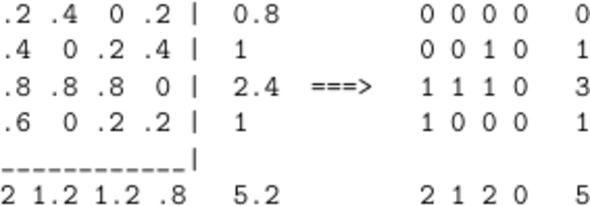
\includegraphics[width=0.5\columnwidth]{figs/table_rounding.pdf}
            \caption{A table rounding examples.}
            \label{fig:table_rounding}
        \end{figure}
        
        Give an efficient algorithm, using network flow, that always finds such
        a rounding. This also provides a proof that such a rounding is always
        possible.
        
        \vspace{10pt}
        \problemAnswer{
            For the original $n$-by-$m$ table $T$, denote its $(j,i)$-th entry
            as $T_{ji}\in[0, 1)$. Define row sum and column sum as
            \begin{align*}
                b_j & = \sum_{i=1}^m T_{ji},\,j=1,\ldots,n \\
                a_i & = \sum_{j=1}^n T_{ji},\,i=1,\ldots,m
            \end{align*}
            respectively, and the total sum as 
            \[
                c = \sum_{j=1}^n b_j = \sum_{i=1}^m a_i =
                \sum_{j=1}^n\sum_{i=1}^m T_{ji}.
            \]
            For a $n$-by-$m$ rounded table $\tilde{T}$, denote its $(j,i)$-th
            entry, the $j$-th row sum, th $i$-th column sum and the total sum as
            $\tilde{T}_{ji}$, $\tilde{b}_j$, $\tilde{a}_i$ and $\tilde{c}$,
            respectively, where
            \begin{align*}
                \tilde{b}_j & = \sum_{i=1}^m \tilde{T}_{ji},\,j=1,\ldots,n \\
                \tilde{a}_i & = \sum_{j=1}^n \tilde{T}_{ji},\,i=1,\ldots,m
            \end{align*}
            and
            \[
                \tilde{c} = \sum_{j=1}^n \tilde{b}_j = \sum_{i=1}^m \tilde{a}_i
                = \sum_{j=1}^n\sum_{i=1}^m \tilde{T}_{ji}.
            \]
            The rounding requirement is then formulated as (from loose to
            tight)
            \begin{subequations}
                \begin{align}
                    & 0 \leq \tilde{T}_{ji} \leq \lceil T_{ji} \rceil \\
                    & \lfloor a_i \rfloor \leq \tilde{a}_i \leq\lceil a_i\rceil,\;
                    \lfloor b_j \rfloor \leq \tilde{b}_j \leq\lceil b_j\rceil \\
                    & \lfloor c \rfloor \leq \tilde{c} \leq\lceil c
                    \rceil.
                \end{align}
                \label{eq:table_round_req}
            \end{subequations}
            This motivates us to build a graph $G = (V, E)$ corresponding to
            the original table, given either $\tilde{c} = \lfloor c \rfloor$ or
            $\tilde{c} = \lceil c \rceil$, where
            \[
                V = \{p\}\cup A \cup B \cup \{q\}
            \]
            in which each node $A_i\in A$, $i=1,\ldots,m$ corresponds to a
            column and each node $B_j\in B$, $j=1,\ldots,n$ corresponds to a
            row. The demands of this nodes are 
            \begin{align*}
                d(A_i) & = -\lfloor a_i \rfloor,\,i=1,\ldots,m \\
                d(B_j) & = \lfloor b_j \rfloor,\,j=1,\ldots,n \\
                d(p) & = -(\tilde{c} - \sum_{i=1}^{m}\lfloor a_i \rfloor) \\
                d(q) & = \tilde{c} - \sum_{j=1}^{n}\lfloor b_j \rfloor
            \end{align*}
            And
            \begin{align*}
                E & =\{(p, A_i)|A_i\in A\} \\ & \cup \{(A_i, B_j)|A_i\in A, B_j\in B\} \\ &
                \cup \{(B_j, q)|B_j\in B\}
            \end{align*}
            over which the capacity is defined as
            \begin{align*}
                c(p, A_i) & = \lceil a_i \rceil - \lfloor a_i \rfloor,\,
                i=1,\ldots,m \\
                c(A_i, B_j) & = \lceil T_{ji} \rceil, \,i=1,\ldots,m, j=1,\ldots,n \\
                c(B_j, q) & = \lceil b_j \rceil - \lfloor b_j \rfloor,\,
                j=1,\ldots,n
            \end{align*}
            An example of graph $G$ is plotted in
            Figure~\ref{fig:table_rounding_G} 
            \begin{figure}[!h]
                \centering
                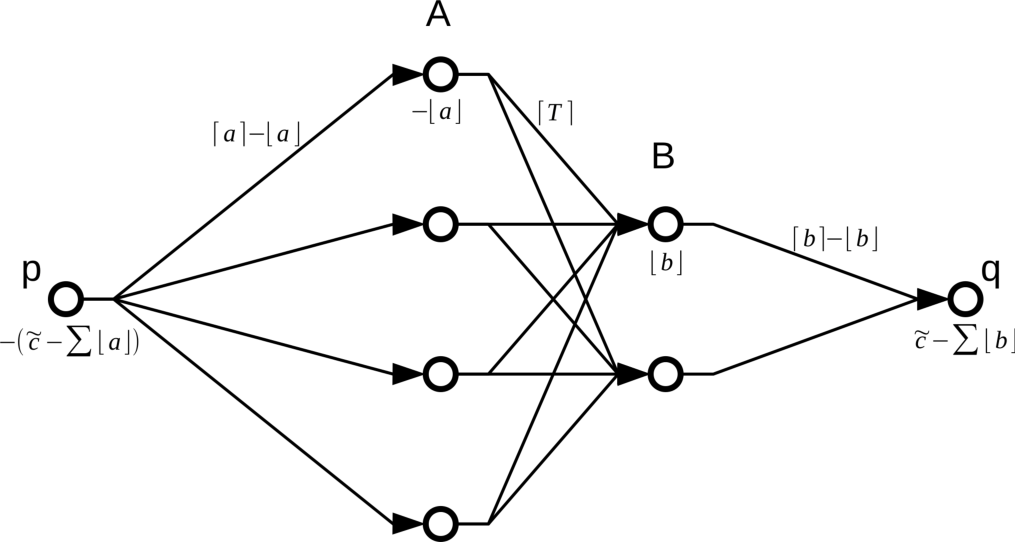
\includegraphics[width=0.5\columnwidth]{figs/table_rounding_G.pdf}
                \caption{Graph $G$ constructed from the original table and
                $\tilde{c}$ where $m=4$ and $n=2$.}
                \label{fig:table_rounding_G}
            \end{figure}
            
            We would like to convert the original table rounding problem into an
            equaivalent circulation with demands problem on $G$ and prove that
            the latter is always feasible and propose an efficient algorithm.
            \begin{lemma}
                There is a one to one mapping between a table rounding scheme
                given $\tilde{c}$ and an integer circulation scheme in graph
                $G$. Given a table rounding scheme specified by $\{\tilde{T}_{ji}\}$,
                $\{\tilde{a}_i\}$, $\{\tilde{b}_j\}$, $\tilde{c}$ corresponds to
                a circulation scheme given by
                \begin{align*}
                    f(p, A_i) &= \tilde{a}_i - \lfloor a_i \rfloor, \, i =
                    1,\ldots, m \\
                    f(A_i, B_j) & = \tilde{T}_{ji},\,i=1,\ldots,m, j=1,\ldots,n \\
                    f(B_j, q) & = \tilde{b}_j - \lfloor b_j \rfloor,\,
                    j=1,\ldots,n
                \end{align*}
                On the other hand, given a feasible integer circulation scheme
                defined by $\{f(p, A_i)\}$, $\{f(A_i,
                B_j)\}$, $\{f(B_j, q)\}$ on $G$, a table rounding scheme is
                given by 
                \begin{align*}
                    \tilde{T}_{ji} & = f(A_i, B_j),\,i=1,\ldots,m,\,j=1,\ldots,n
                    \\
                    \tilde{a}_i &= f(p, A_i) + \lfloor a_i
                    \rfloor,\,i=1,\ldots,m
                    \\
                    \tilde{b}_j &= f(B_j, q) + \lfloor b_j
                    \rfloor,\,j=1,\ldots,n\\
                \end{align*}
                \label{lemma:21}
            \end{lemma}
            \begin{proof}
                (From table rounding to circulation) Firstly it is easy to
                verify that this mapping respects that $0\leq f(u, v) \leq c(u,
                v)$ for all $(u, v)$ in $E$ and all $f(u, v)$ are integers. All
                we need to do is to check the demand conditions: at node $p$, we
                have
                \begin{align*}
                    \sum_{u} f(u, p) - \sum_{v} f(p, v) & = -\sum_{i=1}^{m} f(p,
                    A_i) \\
                    & = - \sum_{i=1}^{m} (\tilde{a}_i -\lfloor{a}_i\rfloor) \\
                    & = - \tilde{c}_i + \sum_{i=1}^{m}\lfloor{a}_i\rfloor \\
                    & = d(p)
                \end{align*}
                at node $A_i$, we have
                \begin{align*}
                    \sum_{u} f(u, A_i) - \sum_{v} f(A_i, v) & = f(p,
                    A_i) - \sum_{j=1}^n f(A_i, B_j)\\
                    & = \tilde{a}_i - \lfloor{a}_i\rfloor - \sum_{j=1}^{n}
                    \tilde{T}_{ji}\\
                    & = - \lfloor{a}_i\rfloor \\
                    & = d(A_i)
                \end{align*}
                According to the symmetric property of graph $G$ and function
                $f$, demand conditions are also satisfied at node $q$ and all
                $B_j$. Consequently, $f$ defines a feasible circulation on $G$.
                \\\\
                (From circulation to table rounding) Firstly we verify that
                $\tilde{T}_{ji}$, $\tilde{a}_i$ $\tilde{b}_j$ are indeed
                roundings of $T_{ji}$, $a_i$ and $b_j$, respectively. Since
                \begin{align*}
                    0\leq f(A_i, B_j) \leq c(A_i, B_j) = \lceil T_{ji} \rceil,
                \end{align*}
                therefore $\tilde{T}_{ji} = f(A_i, B_j)$ is indeed an integer
                round for $T_{ji}\in [0, 1)$. Since
                \begin{align*}
                    \lfloor a_i \rfloor \leq f(p, A_i) + \lfloor a_i \rfloor
                    \leq c(p, A_i) + \lfloor a_i \rfloor = \lceil a_i \rceil
                \end{align*}
                therefore $\tilde{a}_i$ is indded an integer round for $a_i$.
                Similarly we can prove that $\tilde{b}_j$ is indded an integer
                round for $b_j$.
                \\\\
                Next we prove that these roundings $\tilde{T}_{ji}$,
                $\tilde{a}_i$ $\tilde{b}_j$ satisfies the row-sum, column-sum
                and total-sum consistency properties of table rounding. Consider
                the demand condition at node $A_i$, we have
                \begin{align*}
                    \sum_{j=1}^n \tilde{T}_{ji} & = \sum_{j=1}^n f(A_i, B_j) \\
                    & = f(p, A_i) - d(A_i)\\
                    & = f(p, A_i) + \lfloor a_i \rfloor \\
                    & = \tilde{a}_i
                \end{align*}
                so the row-sum consistency is verified. Similarly, by examining
                the demand condition at node $B_j$ we can verify the column-sum
                consistency $\sum_{i=1}^m \tilde{T}_{ji} = \tilde{b}_j$.
                Consider the demand condition at node $p$, we have
                \begin{align*}
                    \sum_{i=1}^m \tilde{a}_i & = \sum_{i=1}^m f(p, A_i) +
                    \sum_{i=1}^m\lfloor a_i \rfloor \\
                    & = -d(p) + \sum_{i=1}^m\lfloor a_i \rfloor \\
                    & = (\tilde{c} - \sum_{i=1}^m\lfloor a_i \rfloor) +
                    \sum_{i=1}^m\lfloor a_i \rfloor \\
                    & = \tilde{c}.
                \end{align*}
                Similarly, by looking at the demand condition at node $q$ we
                have $\sum_{i=1}^m \tilde{b}_j$, therefore the total-sum consistency
                is verified. In conclusion, $\{\tilde{T}_ji\}$ indeed defines a
                valid table rounding scheme.
            \end{proof}
            
            The above lemma suggests that the original table rounding problem is
            equivalent to propose an efficient algorithm to find an integer flow
            with value $\tilde{c}$ in $G$ and prove this flow always exists.
            \begin{lemma}
                The network flow problem on $G$ always have an integer solution
                with value equal to $\tilde{c}$ for either $\tilde{c} = \lfloor c
                \rfloor$ or $\tilde{c} = \lceil c \rceil$.
            \end{lemma}
            \begin{proof}
                According to (7.51) in the text book, we just need to prove
                that for every cut $X, Y$ of $G$:
                \[
                    \sum_{v\in Y} d(v) \leq c(X, Y).
                \]
                Assume
                \[
                    Y = A_Y \cup B_Y \cup H
                \]
                in which $A_Y \subset A$, $B_Y \subset B$ and $H\subset \{p,
                q\}$. Next we prove the above inequality for the 4 different
                $H$:
                \begin{enumerate}
                    \item $H=\{p, q\}$
                    \begin{align*}
                        \sum_{v\in Y} d(v) & = -(\tilde{c} -
                        \sum_{i=1}^{m}\lfloor a_i \rfloor) + (\tilde{c} - \sum_{j=1}^{n}\lfloor b_j
                        \rfloor) - \sum_{A_i\in A_Y}\lfloor a_i \rfloor +
                        \sum_{B_j\in B_Y}\lfloor b_j \rfloor \\
                        & = \sum_{A_i\in A_X} \lfloor a_i \rfloor - \sum_{B_j\in
                        B_X} \lfloor b_j \rfloor \\
                        & \leq \sum_{A_i\in A_X} \tilde{a}_i - \sum_{B_j\in
                        B_X} \lfloor b_j \rfloor \\
                        & = \sum_{A_i\in A_X} \sum_{j=1}^n\tilde{T}_{ji} - \sum_{B_j\in
                        B_X} \lfloor b_j \rfloor \\
                        & \leq \sum_{A_i\in A_X}\sum_{B_j\in B_Y}\tilde{T}_{ji}
                        + \sum_{i=1}^m\sum_{B_j\in B_X} \tilde{T}_{ji} - \sum_{B_j\in
                        B_X} \lfloor b_j \rfloor \\
                        & = \sum_{A_i\in A_X}\sum_{B_j\in B_Y}\tilde{T}_{ji} +
                        \sum_{B_j\in B_X} \tilde{b}_j - \sum_{B_j\in B_X}
                        \lfloor b_j \rfloor \\
                        & \leq \sum_{A_i\in A_X}\sum_{B_j\in B_Y}\lceil T_{ji}
                        \rceil +
                        \sum_{B_j\in B_X} \lceil b_j \rceil - \sum_{B_j\in B_X}
                        \lfloor b_j \rfloor \\
                        & = \sum_{A_i\in A_X}\sum_{B_j\in B_Y}c(A_i, B_j)
                        + \sum_{B_j\in B_X}c(B_j, q) \\
                        & = c(X, Y)
                    \end{align*}
                    \item $H=\{p\}$
                    \begin{align*}
                        \sum_{v\in Y} d(v) & = -(\tilde{c} -
                        \sum_{i=1}^{m}\lfloor a_i \rfloor) - \sum_{A_i\in A_Y}\lfloor a_i \rfloor +
                        \sum_{B_j\in B_Y}\lfloor b_j \rfloor \\
                        & = -\tilde{c} + \sum_{A_i\in A_X} \lfloor a_i \rfloor+
                        \sum_{B_j\in B_Y}\lfloor b_j \rfloor \\
                        & \leq -\tilde{c} + \sum_{A_i\in A_X}\tilde{a}_i
                        +\sum_{B_j\in B_Y}\tilde{b}_j \\
                        & = -\sum_{i=1}^m\sum_{j=1}^n\tilde{T}_{ji} +
                        \sum_{A_i\in A_X}\sum_{j=1}^n\tilde{T}_{ji} + 
                        \sum_{i=1}^m\sum_{B_j\in B_Y}\tilde{T}_{ji} \\
                        & \leq \sum_{A_i\in A_X}\sum_{B_j\in B_Y}\tilde{T}_{ji}
                        \\
                        & \leq \sum_{A_i\in A_X}\sum_{B_j\in B_Y} \lceil T_{ji}
                        \rceil \\
                        & = \sum_{A_i\in A_X}\sum_{B_j\in B_Y}c(A_i, B_j)\\
                        & = c(X, Y)
                    \end{align*}
                    \item $H=\{q\}$
                    \begin{align*}
                        \sum_{v\in Y} d(v) & = - \sum_{A_i\in A_Y}\lfloor a_i
                        \rfloor + \sum_{B_j\in B_Y}\lfloor b_j \rfloor +
                        (\tilde{c} - \sum_{j=1}^n\lfloor b_j \rfloor) \\
                        & = \tilde{c} - \sum_{A_i\in A_Y}\lfloor a_i \rfloor -
                        \sum_{B_j\in B_X}\lfloor b_j \rfloor \\
                        & = \sum_{i=1}^m\sum_{j=1}^n\tilde{T}_{ji} -
                        \sum_{A_i\in A_Y}\lfloor a_i \rfloor - \sum_{B_j\in
                        B_X}\lfloor b_j \rfloor \\
                        & \leq \sum_{A_i\in A_Y}\sum_{j=1}^n \tilde{T}_{ji} +
                        \sum_{i=1}^m\sum_{B_j\in B_X} \tilde{T}_{ji} +
                        \sum_{A_i\in A_X}\sum_{B_j\in B_Y} \tilde{T}_{ji} -
                        \sum_{A_i\in A_Y}\lfloor a_i \rfloor - \sum_{B_j\in
                        B_X}\lfloor b_j \rfloor \\
                        & = \sum_{A_i\in A_Y} \tilde{a}_i + \sum_{B_j\in B_X}
                        \tilde{b}_j + \sum_{A_i\in A_X}\sum_{B_j\in B_Y}
                        \tilde{T}_{ji} -
                        \sum_{A_i\in A_Y}\lfloor a_i \rfloor - \sum_{B_j\in
                        B_X}\lfloor b_j \rfloor \\
                        & \leq \sum_{A_i\in A_Y}(\lceil a_i \rceil - \lfloor
                        a_i \rfloor) + \sum_{A_i\in A_X}\sum_{B_j\in B_Y}
                        \lceil T_{ji} \rceil + \sum_{B_j\in B_X}(\lceil b_j
                        \rceil - \lfloor b_j \rfloor) \\
                        & = \sum_{A_i\in A_Y}c(p, A_i) + \sum_{A_i\in
                        A_X}\sum_{B_j\in B_Y}c(A_i, B_j) + \sum_{B_j\in
                        B_X}c(B_j, q) \\
                        & = c(X, Y)
                    \end{align*}
                    \item $H = \emptyset$
                    \begin{align*}
                        \sum_{v\in Y} d(v) & = -\sum_{A_i\in A_Y}\lfloor a_i
                        \rfloor + \sum_{B_j\in B_Y}\lfloor b_j \rfloor \\
                        & \leq -\sum_{A_i\in A_Y}\lfloor a_i \rfloor
                        + \sum_{B_j\in B_Y}\tilde{b}_j \\
                        & = -\sum_{A_i\in A_Y}\lfloor a_i \rfloor +
                        \sum_{i=1}^m\sum_{B_j\in B_Y} \tilde{T}_{ji} \\
                        & \leq -\sum_{A_i\in A_Y}\lfloor a_i \rfloor +
                        \sum_{A_i\in A_Y}\sum_{j=1}^n \tilde{T}_{ji} +
                        \sum_{A_i\in A_X}\sum_{B_j\in B_Y} \tilde{T}_{ji}\\
                        & = -\sum_{A_i\in A_Y}\lfloor a_i \rfloor + \sum_{A_i\in
                        A_Y} \tilde{a}_i + \sum_{A_i\in A_X}\sum_{B_j\in B_Y}
                        \tilde{T}_{ji} \\
                        & \leq \sum_{A_i\in A_Y} (\lceil a_i \rceil - \lfloor
                        a_i \rfloor) + \sum_{A_i\in A_X}\sum_{B_j\in B_Y} \lceil
                        T_{ji} \rceil \\
                        & = \sum_{A_i\in A_Y}c(p, A_i) + \sum_{A_i\in
                        A_X}\sum_{B_j\in B_Y}c(A_i, B_j) \\
                        & = c(X, Y)
                    \end{align*}
                \end{enumerate}
            \end{proof}
            From the above lemma, the circulation with demands problem is always
            feasible, indicating that the equivalent table rounding problem is
            always feasible. For an efficient algorithm to solve the table
            rounding problem, we can further extend graph $G$ to $G'$ by adding
            a source node $s$, a sink node $t$ and the corresponding edges
            $(s,p)$, $(s,  A_i)$, $(B_j, t)$ and $(q, t)$, as described in the
            text book. An example of $G'$ is shown in
            Figure~\ref{fig:table_rounding_network}. We can use the
            Ford-Fulckerson algorithm to find a integer flow with value
            $\tilde{c}$ in $G'$, then the table rounding scheme is defined as in
            Lemma~\ref{lemma:21}.
            
            \begin{figure}[!h]
                \centering
                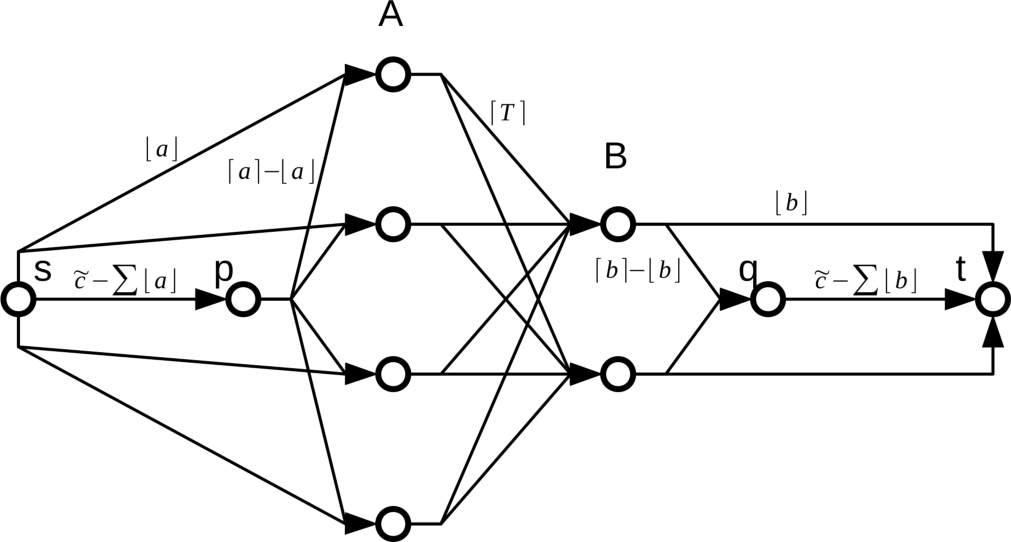
\includegraphics[width=0.6\columnwidth]{figs/table_rounding_network.pdf}
                \caption{Graph $G'$ based on the circulation problem.}
                \label{fig:table_rounding_network}
            \end{figure}
            
        }
        
    \end{homeworkProblem}
    
    %----------------------------------------------------------------------------------------
    %   PROBLEM 3
    %----------------------------------------------------------------------------------------
    \begin{homeworkProblem}
        Suppose $(X, Y)$ and $(X', Y')$ are two distinct minimum-capacity $s$,
        $t$ cuts in a directed network $G$. Prove that $(X\cup X' , Y\cap Y')$
        and $(X\cap X' , Y\cup Y')$ are also a minimum-capacity $s$, $t$ cuts in
        $G$. The key to this problem is to remember that an $s$, $t$ cut is a
        partition of the nodes with $s$ in one subset and $t$ in the other, so
        there are four subsets of nodes when you examine $X$, $Y$, $X'$, $Y'$
        together; then do a case analysis by looking closely at the capacities
        of the edges from one subset of nodes to another.
        
        \vspace{10pt}
        \problemAnswer{
            It is apparent that both $(X\cup X' , Y\cap Y')$ and $(X\cap X',
            Y\cup Y')$ are partitions of $V = X\cup Y = X'\cup Y'$ as $X\cap Y =
            X'\cap Y' = \emptyset$. Also as $s\in X$ and $s\in X'$, we have
            $s\in X\cap X'$ and $s\in X\cup X'$ and similarly $t\in Y\cap Y'$
            and $t\in Y\cup Y'$, which means both $(X\cup X' , Y\cap Y')$ and
            $(X\cap X' , Y\cup Y')$ are indeed $s,t$ cuts. Since $(X, Y)$ and
            $(X', Y')$ are min-cut, we have
            \begin{align*}
                c(X\cup X', Y\cap Y') & \geq c(X, Y) = c(X', Y') \\
                c(X\cap X', Y\cup Y') & \geq c(X, Y) = c(X', Y').
            \end{align*}
            As a result,
            \begin{align*}
                c(X\cup X', Y\cap Y') + c(X\cap X', Y\cup Y') \geq c(X, Y) +
                c(X', Y')
            \end{align*}
            the equality holds iff $(X\cup X' , Y\cap Y')$ and $(X\cap X' ,
            Y\cup Y')$ are both min-cut. On the other hand
            \begin{align*}
                & c(X\cup X', Y\cap Y') + c(X\cap X', Y\cup Y') \\
                &=\sum_{u\in X\backslash X'}\sum_{v\in Y\cap Y'}c(u, v)
                +\sum_{u\in X'\backslash X}\sum_{v\in Y\cap Y'}c(u, v)
                +\sum_{u\in X\cap X'}\sum_{v\in Y\cap Y'}c(u, v) \\
                &+\sum_{u\in X\cap X'}\sum_{v\in Y\backslash Y'}c(u, v)
                +\sum_{u\in X\cap X'}\sum_{v\in Y'\backslash Y}c(u, v)
                +\sum_{u\in X\cap X'}\sum_{v\in Y\cap Y'}c(u, v) \\
                & \leq \sum_{u\in X\backslash X'}\sum_{v\in Y\backslash Y'}c(u,
                v)
                +\sum_{u\in X\backslash X'}\sum_{v\in Y\cap Y'}c(u, v)
                +\sum_{u\in X\cap X'}\sum_{v\in Y\backslash Y'}c(u, v)
                +\sum_{u\in X\cap X'}\sum_{v\in Y\cap Y'}c(u, v) \\
                &+ \sum_{u\in X'\backslash X}\sum_{v\in Y'\backslash Y}c(u,
                v)
                +\sum_{u\in X'\backslash X}\sum_{v\in Y'\cap Y}c(u, v)
                +\sum_{u\in X'\cap X}\sum_{v\in Y'\backslash Y}c(u, v)
                +\sum_{u\in X'\cap X}\sum_{v\in Y'\cap Y}c(u, v) \\
                &= c(X, Y) + c(X', Y')
            \end{align*}
            Consequently, $c(X\cup X', Y\cap Y') + c(X\cap X', Y\cup Y') = c(X,
            Y) + c(X', Y')$. Thus
            \begin{align*}
                c(X\cup X', Y\cap Y') = c(X\cap X', Y\cup Y') = c(X, Y) = c(X',
                Y') \\
            \end{align*}
            i.e. both $(X\cup X' , Y\cap Y')$ and $(X\cap X' , Y\cup Y')$ are
            min-cap $s,t$ cut in $G$.
        }
    \end{homeworkProblem}
    %\clearpage
    
    %----------------------------------------------------------------------------------------
    %   PROBLEM 4
    %----------------------------------------------------------------------------------------
    \begin{homeworkProblem}
         In some applications of numerical linear algebra you are given a sparse
         square matrix $M$ (say $n$ by $n$) and you want to permute the rows and
         columns of $M$ so that the main diagonal has no 0, if possible. Show
         how to find such a permutation, if there is one, by using network flow.
         Hint: The key here is to use network flow to find a set of $n$ non-zero
         entries in $M$ such that no two are in the same row or column. For the
         network, start with a bipartite graph to represent the non-zero
         entries of $M$, and then add the $s$ and $t$ nodes.
        
        
        \vspace{10pt}
        \problemAnswer{
            \begin{lemma}
                Given 2 entries $M_{i_1j_1}$ and $M_{i_2j_2}$ such that
                $i_1\not=i_2$ and $j_1\not=j_2$. Suppose after an arbitrary
                series of row permutations and column permutations, this 2
                entries are moved to $M_{i_1'j_1'}$ and $M_{i_2'j_2'}$, then we
                still have $i_1'\not=i_2'$ and $j_1'\not=j_2'$.
            \end{lemma}
            \begin{proof}
                If is sufficient to prove that after a single row-swap we still
                have $i_1'\not=i_2'$ and $j_1'\not=j_2'$. Then the conclusion
                can be generalized to a single column swap due to symmertry and
                generalized to arbitrary row/column permutattions according to
                mathematical induction.
                \begin{itemize}
                    \item If row $i_1$ and row $i_2$ are swapped, then $i_1' =
                    i_2$, $j_1' = j_1$, $i_2' = i_1$, $j_2' = j_2$, the 2
                    inequalities hold.
                    \item If row $i_1$ is swapped with row $i_3\not=i_2$, then
                    $i_1' = i_3$, $j_1' = j_1$, $i_2' = i_2$, $j_2' = j_2$, the
                    2 inequalities hold.
                    \item If 2 rows are swapped but neither $i_1$-th row nor
                    $i_2$-th row is involved, the 2 entries are not moved at
                    all, so the 2 inequalities still hold.
                \end{itemize}
                \label{lemma:41}
            \end{proof}
            
            \begin{corollary}
                If we can find a permutation so that the diagonal elements of
                $M$ is non-zero, then we must be able to find a set of non-zero
                entries in the original $M$ such that no 2 entries are in the
                same row or column.
            \end{corollary}
            \begin{proof}
                We note that the row and column permutations are invertible.
                Since in the resulting matrix $M'$ we have $n$ non-zero diagonal
                elements, and obviously any pair of them are in different rows
                and columns, according to Lemma~\ref{lemma:41} in the orignal
                matrix $M$ this $n$ non-zero entries satisfy the property that
                no 2 of them are in the same row or column.
            \end{proof}
            Algorithm~\ref{alg:perm} is able to find such a
            permutation given the $n$ non-zero elements among which there are no
            2 entries in the same row or column. Consequently, finding the
            permutation and finding the $n$ non-zero elements are equivalent
            problems.
            \begin{algorithm}
                \caption{$perm(M)$: the function to permute the rows and
                columns in $n$-by-$n$ matrix $M$ so that all diagonal entries
                are non-zero, suppose there are a list of $n$ non-zero entries
                $L = \{M_{i_1j_1},\ldots,M_{i_nj_n}\}$ in $M$ among which no two
                are in the same row or column.}
                \label{alg:perm}
                \begin{algorithmic}[1]
                    \IF {$n=1$}
                        \RETURN
                    \ELSIF {$M_{11} \notin L$}
                        \STATE Swap row 1 and row $i_1$.
                        \STATE Swap column 1 and column $j_1$.
                    \ENDIF
                    \STATE Call $perm(M_{2:n, 2:n})$.
                \end{algorithmic}
            \end{algorithm}
            This recursive algorithm is valid since after step 3-6, we have made
            sure that $M_{11}\not = 0$. According to Lemma~\ref{lemma:41}, all
            the remaining $n-1$ entries in $L$ is now in $M_{2:n, 2:n}$ and
            still no two of them are in the same row or column.
            
            To find such $n$ non-zero entries in $M$,
            we construct a table $G=(V, E)$ as follows:
            \begin{itemize}
                \item $V = \{s\} \cup A \cup B \{t\}$, where $s$, $t$ are the
                source and the sink node respectively, $A = \{A_i|i=1,\ldots,
                n\}$ corresponds to the $n$ rows and $B = \{B_j|j=1,\ldots,
                n\}$ corresponds to the $n$ columns.
                \item $E = \{(s, A_i\}\cup\{(A_i,B_j)\}\cup\{(B_j, t)\}$, where
                $c(s, A_i) = 1, i=1,\ldots,n$, $c(B_j, t) = 1, j=1,\ldots,n$,
                $c(A_i,B_j) = 1$ if $M_{ij}\not=0$ and $c(A_i,B_j) = 0$
                otherwise.
            \end{itemize}
            \begin{lemma}
                There is a one-to-one mapping between a list of $n$ non-zero entries
                $L = \{M_{i_1j_1},\ldots,M_{i_nj_n}\}$ in $M$ among which no two
                are in the same row or column, and an integer flow on $G$
                with value $n$.
                \label{lemma:43}
            \end{lemma}
            \begin{proof}
                (From $L$ to flow) Given the non-zero entries list $L =
                \{M_{i_1j_1},\ldots,M_{i_nj_n}\}$, we define a flow in $G$ as
                \begin{align*}
                    f(s, A_i) & = 1,\, i = 1,\ldots,n \\
                    f(A_i, B_j) & = \left\{\begin{array}{ll}1
                    & \mbox{if } M_{ij}\in L \\ 0 &
                    \mbox{else.}\end{array}\right. ,\, i,j=1,\ldots,n\\
                    f(B_j, t) &= 1,\, j=1,\ldots, n
                \end{align*}
                Firstly it is easy to verify that $0\leq f(u, v) \leq c(u, v)$
                for all $(u, v)\in E$. Consider the conservation law at node
                $A_i$. Since no 2 indices in $\{i_1,\ldots,i_n\}$ are the same,
                $\{i_1,\ldots,i_n\}$ must be a permutation of $1,\ldots,n$,
                consequently, there is exactly one non-zero flow $f(A_i, B_j)=1$
                from $A_i$. Also there is exactly one flow $f(s, A_i)=1$.
                Therefore the convervation law holds at any node $A_i$. Due to
                symmetric structure of $G$, it is easy to verify that the
                conservation law also holds for any node $B_j$. In conclusion,
                function $f$ defined above is indeed a flow in $G$.
                \\\\
                (From flow to $L$) Firstly we show that an integer flow on $G$
                with value $n$ must satisfy the following properties:
                \begin{itemize}
                    \item $f(s, A_i)=f(B_j, t) = 1$, $i,j = 1,\ldots,n$. By
                    considering the cut $(\{s\}, V\backslash\{s\})$, we have
                    \begin{align*}
                        n = f(\{s\}, V\backslash\{s\}) \leq c(\{s\},
                        V\backslash\{s\}) = n
                    \end{align*}
                    therefore $(\{s\}, V\backslash\{s\})$ is indeed a
                    min-cut and each edge $(s, A_i)$ must be saturated.
                    Similarly, by considering the cut $(V\backslash\{t\},
                    \{t\})$, each edge $(B_j, t)$ must also be saturated.
                    \item For any node $A_i$, there exists exactly one
                    $B_{j(i)}$ such that $f(A_i, B_{j(i)}) = 1$ and all other
                    edges out from $A_i$ have 0 flow on them. Conversely, for
                    any node $B_j$, there exists exactly one $A_{i(j)}$ such
                    that $f(A_{i(j)}, B_j) = 1$ and all other edges into $B_j$
                    have 0 flow on them. This is because at node $A_i$, we have
                    \begin{align*}
                        \sum_{j=1}^n f(A_i, B_j) = f(s, A_i) = 1
                    \end{align*}
                    while at node $B_j$, we have
                    \begin{align*}
                        \sum_{i=1}^n f(A_i, B_j) = f(B_j, t) = 1
                    \end{align*}
                    and $f(A_i, B_j)$ must be integer.
                \end{itemize}
                Consequently, from such an integer flow with value $n$, we can
                simply build $L=\{M_{1,j(1)},\ldots,M_{n,j(n)}\}$ and it is
                guaranteed that no 2 indices in $j(1),\ldots,j(n)$ are equal.
            \end{proof}
            
            According to Lemma~\ref{lemma:43}, the original problem is
            equivalent to finding an integer flow with value $n$ in $G$. Also if
            such a flow exist it must be a max-flow since $c(\{s\},
            V\backslash\{s\}) = n$. Therefore, to find $L =
            \{M_{i_1j_1},\ldots,M_{i_nj_n}\}$ we can simply run the
            Ford-Fulkerson algorithm on $G$. If the resulting integer max-flow
            has value $n$, then we build $L$ as described in the proof of
            Lemma~\ref{lemma:43}, and use Algorithm~\ref{alg:perm} to execute
            the permutations.
            
        }
     
    \end{homeworkProblem}
    %\clearpage
    
    %----------------------------------------------------------------------------------------
    %   PROBLEM 5
    %----------------------------------------------------------------------------------------
    \begin{homeworkProblem}
        
         Show that if $f$ is some non-maximum $s-t$ flow in a graph $G$, and
         $G_f$ is the residual graph with respect to $f$, then flow $f$
         \emph{superimposed} with a maximum $s-t$ flow $g$ in $G_f$ is a maximum
         flow in $G$. By superposition we mean the addition of the two flows;
         however if for an edge $(i,j)$ there is flow from $i$ to $j$ in $f$ and
         flow from $j$ to $i$ in $g$ (recall that $g$ is a flow in $G_f$ so that
         this is possible, since $(j,i)$ is a backward edge) then the
         superposition of these flows means the subtraction of $g(j,i)$ from
         $f(i,j)$. That is, forward flows in $f$ and $g$ are added, but a
         backward flow in $g$ is subtracted from the corresponding forward flow
         in $f$.
        
        \vspace{10pt}
        \problemAnswer{
                
        }
     
    \end{homeworkProblem}
    %\clearpage
    
    %----------------------------------------------------------------------------------------

\end{document}